%==============================================================================
% Sjabloon poster bachproef
%==============================================================================
% Gebaseerd op document class `a0poster' door Gerlinde Kettl en Matthias Weiser
% Aangepast voor gebruik aan HOGENT door Jens Buysse en Bert Van Vreckem

\documentclass[a0,portrait]{hogent-poster}

% Info over de opleiding
\course{Bachelorproef}
\studyprogramme{toegepaste informatica}
\academicyear{2025-2026}
\institution{Hogeschool Gent, Valentin Vaerwyckweg 1, 9000 Gent}

% Info over de bachelorproef
\title{Automatisatie van het onboarding- en offboardingsproces binnen het gemeentebestuur van Berlare}
\author{Ewout Van Mullem}
\email{ewout.vanmullem@student.hogent.be}
\supervisor{Thomas Aelbrecht}
\cosupervisor{Hans Van Mingeroet (Gemeentebestuur Berlare)}

% Indien ingevuld, wordt deze informatie toegevoegd aan het einde van de
% abstract. Zet in commentaar als je dit niet wilt.
\specialisation{Systeem- en Netwerkbeheer}
\keywords{Onboarding, Offboarding, Procesautomatisatie, IT-automatisatie, Gebruikersbeheer, Identiteits- en toegangsbeheer, Gemeentebestuur, IT-beheer}
\projectrepo{https://github.com/Ewout-VM/VanMullemEwout-BP}

\begin{document}

\maketitle

% \begin{abstract}
% Deze bachelorproef onderzoekt de automatisatie van het onboarding- en offboardingproces binnen de IT-infrastructuur van het gemeentebestuur van Berlare. De oorspronkelijke processen verliepen grotendeels manueel, waardoor ze tijdrovend waren en gevoelig voor menselijke fouten.

% Op basis van een analyse van de bestaande processen en IT-infrastructuur werd een automatiseringsoplossing ontwikkeld met Microsoft Power Automate, PowerShell en Microsoft 365-diensten. Hiermee worden gebruikers automatisch aangemaakt, geconfigureerd en uit dienst genomen. Ook het toekennen en verwijderen van rechten, licenties, mailboxrechten en distributiegroepen wordt geautomatiseerd.

% De oplossing vermindert repetitieve handelingen, verkleint de kans op configuratiefouten en zorgt voor een snellere en meer consistente verwerking van medewerkers. Het onderzoek toont aan dat automatisatie een duidelijke meerwaarde biedt binnen een lokaal bestuur met een hybride IT-omgeving. De werking blijft wel afhankelijk van correcte invoergegevens, een goed beheerde rechtenstructuur en regelmatig onderhoud.

% \end{abstract}

\begin{multicols}{2} % This is how many columns your poster will be broken into, a portrait poster is generally split into 2 columns

\section{Introductie}

Binnen het gemeentebestuur van Berlare verlopen het onboarding- en offboardingproces van medewerkers grotendeels manueel. IT-medewerkers moeten hierbij verschillende handelingen uitvoeren in onder andere Active Directory, Entra ID en Microsoft 365.

Deze werkwijze zorgt voor een hoge administratieve belasting, tijdverlies en een verhoogd risico op menselijke fouten, ontbrekende configuraties en laattijdige acties.

Daarom werd onderzocht hoe deze processen binnen de bestaande hybride IT-omgeving geautomatiseerd en consistenter uitgevoerd kunnen worden.
\section{Onderzoeksvraag}

Op welke manier kan een geautomatiseerd systeem ontwikkeld worden dat, op basis van gegevens uit de personeelsdienst, een volledige en correcte onboarding en offboarding kan uitvoeren binnen de IT-infrastructuur van het gemeentebestuur van Berlare?

% \section{Sectie met figuur}

% De {\LaTeX} figure-omgeving bepaalt zelf waar een afbeelding komt en dat is meestal niet op de plek in de tekst waar de figure-omgeving gedefinieerd wordt. Als je wilt forceren dat afbeeldingen toch in de flow van de tekst blijven, dan kan je dat zoals hieronder:

% \begin{center}
%   \captionsetup{type=figure}
%   
\includegraphics[width=1.0\linewidth]{grail}
%   \captionof{figure}{He hasn't got shit all over him. The nose? Where'd you get the coconuts? What do you mean? We shall say `Ni' again to you, if you do not appease us}
% \end{center}

% Let er wel op dat dit tot problemen met bladschikking kan leiden.

\section{Methodologie}

Het onderzoek werd uitgevoerd aan de hand van een Proof of Concept-methode,
waarbij de oplossing iteratief werd ontworpen, ontwikkeld en geëvalueerd.

\subsection{Analyse}
Het bestaande onboarding- en offboardingproces en de IT-infrastructuur
werden geanalyseerd. Hierbij werden knelpunten en mogelijke
automatiseringsstappen geïdentificeerd.

\subsection{Ontwerp}
Op basis van de analyse werd een geautomatiseerde workflow ontworpen
voor de bestaande hybride IT-omgeving.

\subsection{Implementatie}
De oplossing werd gerealiseerd met Microsoft Forms, Power Automate,
Power Automate Desktop, PowerShell en Microsoft 365.

\subsection{Evaluatie}
De geautomatiseerde processen werden vergeleken met de oorspronkelijke
manuele werkwijze op vlak van tijd, efficiëntie, consistentie en
betrouwbaarheid.
% \section{Toekomstig onderzoek}

% I care. So, what do you think of her, Han? No! Alderaan is peaceful. We have no weapons. You can't possibly… I have traced the Rebel spies to her. Now she is my only link to finding their secret base.

% Kid, I've flown from one side of this galaxy to the other. I've seen a lot of strange stuff, but I've never seen anything to make me believe there's one all-powerful Force controlling everything. There's no mystical energy field that controls my destiny. It's all a lot of simple tricks and nonsense. You are a part of the Rebel Alliance and a traitor! Take her away! 

\section{Gerealiseerde oplossing}

% \begin{center}
%   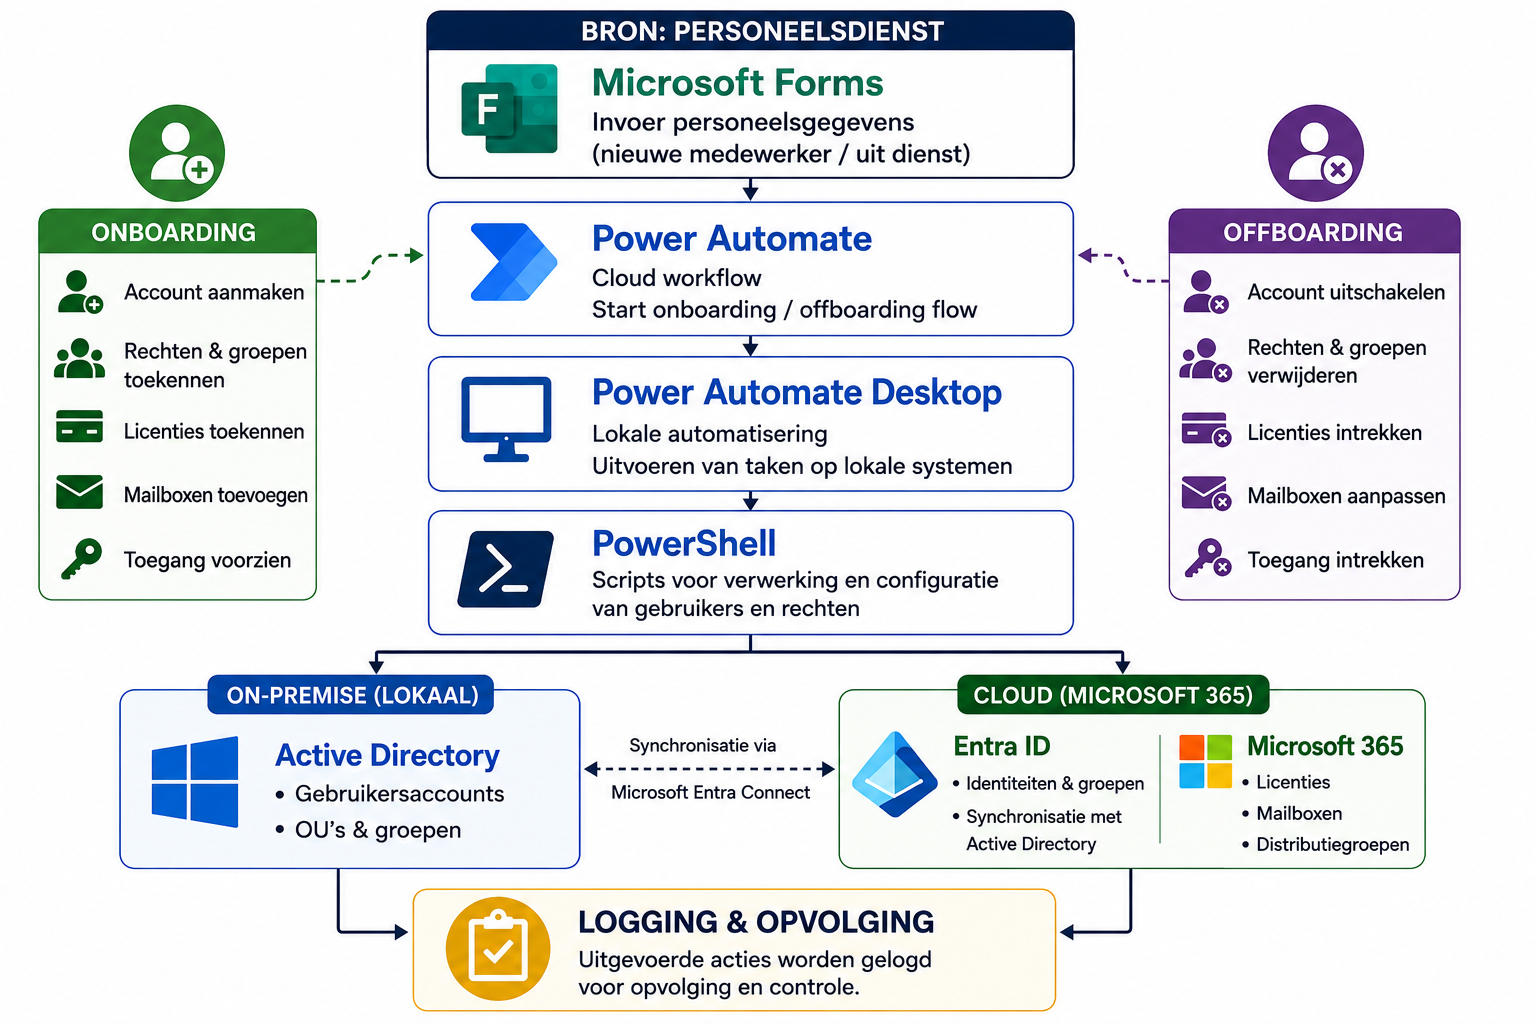
\includegraphics[width=1.0\linewidth]{graphics/Uitwerking.png}

%   \captionsetup{type=figure}
%   \captionof{figure}{Visuele voorstelling van het uitgewerkte proces}
% \end{center}

\begin{minipage}{\linewidth}
    \centering
    \hspace*{-0.15\linewidth}
    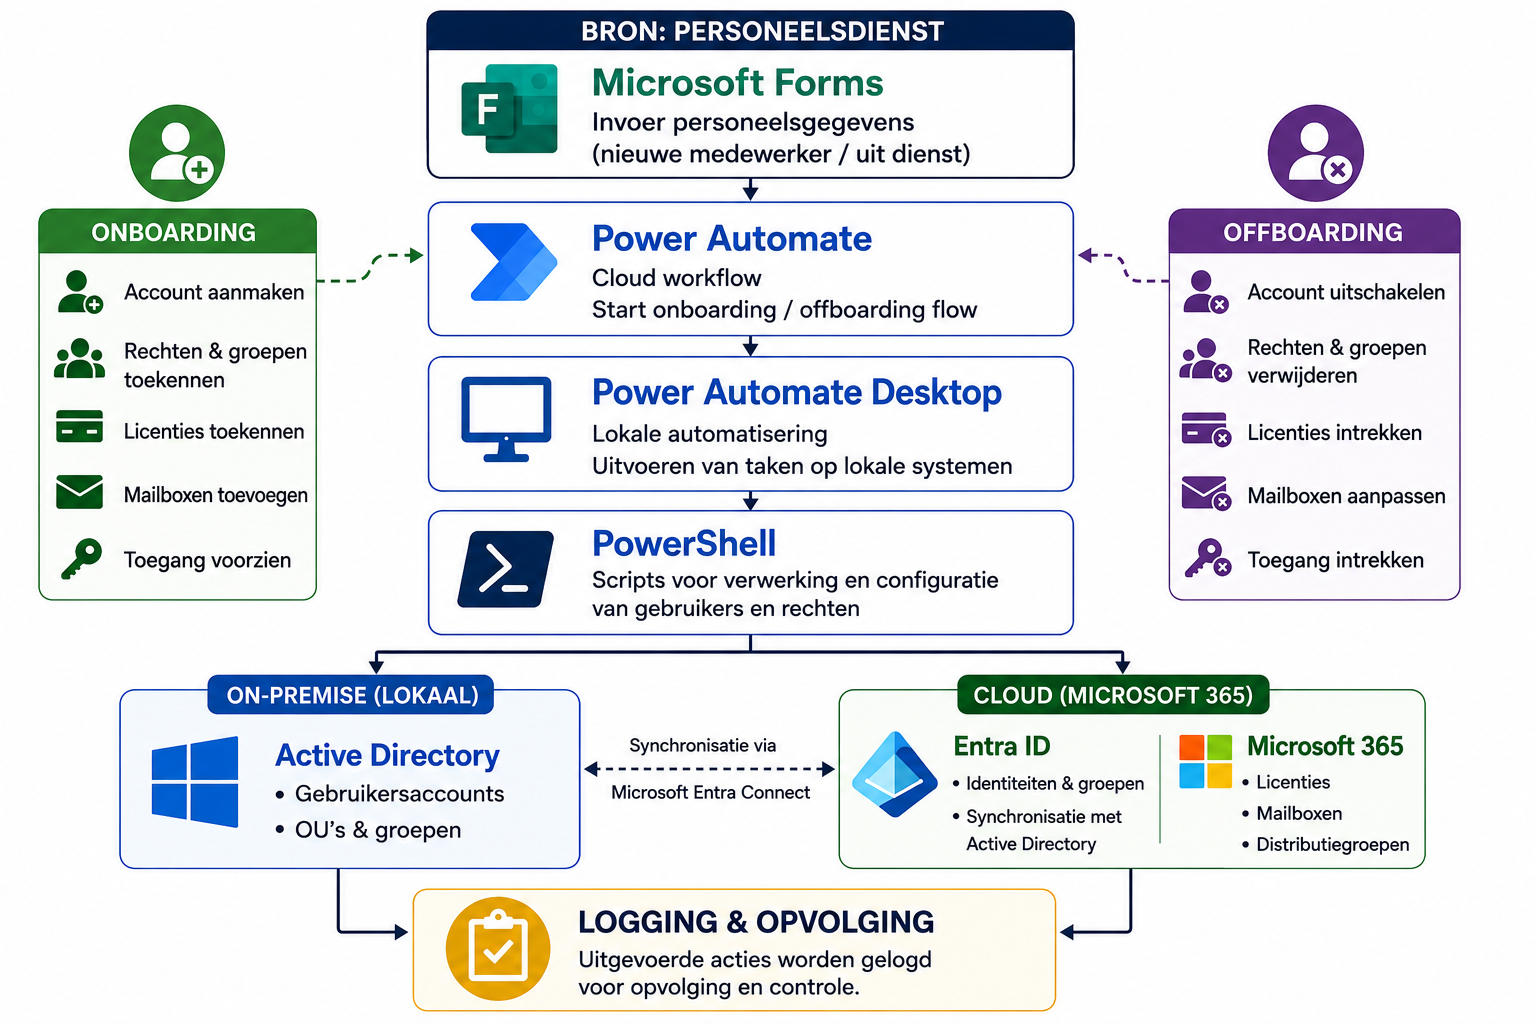
\includegraphics[width=1.15\linewidth,height=30cm]{graphics/Uitwerking.png}
    
    \captionof{figure}{Visuele voorstelling van het uitgewerkte proces}
\end{minipage}

\section{Resultaten}

% De ontwikkelde automatisering werd getest binnen de bestaande hybride IT-omgeving van het gemeentebestuur van Berlare.

% Repetitieve taken binnen onboarding en offboarding worden automatisch uitgevoerd, waardoor de IT-dienst minder handmatig werk moet verrichten.

% Gebruikers worden volgens vooraf bepaalde regels aangemaakt, toegewezen aan de juiste OU's en groepen en voorzien van de benodigde rechten en licenties.

% De automatisering verkort de verwerking van gebruikers en maakt het mogelijk om meerdere opeenvolgende stappen automatisch uit te voeren.

% Uitgevoerde acties worden bijgehouden, waardoor de voortgang van het proces beter gecontroleerd en opgevolgd kan worden.

De ontwikkelde automatisering werd getest binnen de bestaande hybride
IT-omgeving van het gemeentebestuur van Berlare. De automatisering vermindert de actieve verwerkingstijd van onboarding
van 13--21 minuten naar 2--3 minuten en beperkt het aantal manuele handelingen.

\begin{center}

\setlength{\fboxsep}{12pt}

\fbox{
  \parbox{0.90\linewidth}{
    \centering

    \textbf{\large Onboarding: actieve verwerkingstijd}

    \vspace{8pt}

    \begin{tabular}{c@{\hspace{25pt}}c@{\hspace{25pt}}c}

      \textbf{Manueel} & & \textbf{Geautomatiseerd} \\[3pt]

      \textbf{\Large 13--21 min.} &
      \textbf{\Large $\rightarrow$} &
      \textbf{\Large 2--3 min.}

    \end{tabular}

    \vspace{6pt}

    \textit{10--19 minuten minder actieve verwerkingstijd}

  }
}

\end{center}

\vspace{8pt}

\subsection{Bereikte automatisering}

\begin{tabular}{p{0.46\linewidth} p{0.46\linewidth}}
\textbf{Onboarding} &
\textbf{Offboarding} \\[4pt]

$\bullet$ Gebruiker automatisch aangemaakt &
$\bullet$ Account automatisch gedeactiveerd \\

$\bullet$ OU's en groepen automatisch bepaald &
$\bullet$ Groepen automatisch verwijderd \\

$\bullet$ Licenties automatisch toegewezen &
$\bullet$ Licenties automatisch ingetrokken \\

$\bullet$ Mailboxrechten automatisch verwerkt &
$\bullet$ Mailboxrechten automatisch verwijderd \\

$\bullet$ Automatische logging &
$\bullet$ Automatische verwerking op einddatum
\end{tabular}

\vspace{8pt}

\subsection{Betrouwbaarheid}

Gegevens worden één keer ingevoerd via Microsoft Forms en vervolgens
automatisch verwerkt volgens vaste mappings en regels. Hierdoor worden
manuele configuratiestappen verminderd en neemt de kans op vergeten of
inconsistente configuraties af.

Daarnaast zorgen logging, foutafhandeling en automatische
herhalingsmechanismen voor een betere opvolging en betrouwbaarheid van
het proces.

\section{Conclusie}

De ontwikkelde oplossing toont aan dat het onboarding- en offboardingproces binnen het gemeentebestuur van Berlare succesvol kan worden geautomatiseerd binnen de bestaande hybride IT-omgeving.

Door de inzet van Power Automate, Power Automate Desktop en PowerShell worden repetitieve handelingen verminderd en kunnen gebruikers consistenter en efficiënter worden verwerkt. Hierdoor wordt de IT-dienst ontlast en neemt de betrouwbaarheid van beide processen toe.

De oplossing vormt bovendien een basis voor verdere automatisering en integratie binnen de IT-omgeving.

\section{Beperkingen \& toekomst}
Hardware, specifieke toegangsrechten en bepaalde Exchange Online-configuraties blijven deels manueel. Verdere integratie en certificaatgebaseerde authenticatie bieden mogelijkheden voor uitbreiding.

\end{multicols}
\end{document}